\documentclass[a4paper,12pt]{article}
%\usepackage{stdpage}
\usepackage{microtype}
\usepackage{tikz}
\usetikzlibrary{calc}
\usetikzlibrary{through}
\usepackage{tgpagella}
\usepackage{subfig}
\usepackage[utf8]{inputenc}
\usepackage[unicode,breaklinks=true,hypertexnames=false]{hyperref}

\definecolor{mylinkcolor}{rgb}{0,0,0.5}
\hypersetup{%
   colorlinks=true,%
   linkcolor=mylinkcolor,%
   urlcolor=mylinkcolor,%
}

\begin{document}

\section{Summary}

This document describes the usage and implementation of two games for
multi-touch tables, Maze and Towers, a utility for replaying past games to
help analyze players' behavior, and a multi-touch table built for testing the
games.

\subsection{Used Abbreviations}

FTIR: Frustrated total internal reflection
LCD: Liquid crystal display
LED: Light emitting diode

\section{Installation}

Before software is installed, it is necessary to ensure that a multi-touch
table is available.
For “homemade” optical multitouch tables, such as the one described in
section \ref{hw}, a TUIO server must also be installed and calibrated.
Available open source TUIO servers include \emph{Community Core Vision} and
Movid.
% XXX: HOMEPAGES!
Refer to the server's documentation for setup instructions for different
operating systems.

Before installing the games themselves, the following dependencies must be
set up according to instructions on their respective home pages, depending
on the operating system:

\begin{itemize}
\item Python (python.org)
\item Setuptools % XXX: HOMEPAGE!
\item Kivy (kivy.org)
\item Cython % XXX: HOMEPAGE!
\item Numpy % XXX: HOMEPAGE!
\end{itemize}

The dependencies are further desribed in section \ref{dependencies}.

The games may be downloaded, or cloned using the version control system Git,
from \url{http://github.com/encukou/touchgames}.

After downloading, the games may be installed using the command
\texttt{python setup.py install}.

\section{User manual}

The games and utility may be run as Python modules from the command line as
\texttt{python -m touchgames.maze}, or
\texttt{python -m touchgames.towers}, or
\texttt{python -m touchgames.replay <filename>} for Maze, Towers and the replay
script, respectively.

Alternatively, on most operating systems it will be possible to double-click
the game module (\texttt{maze.py} or \texttt{towers.py}) to run the
corresponding game.

\subsection{Maze}

The Maze game is played by two players, the \emph{Solver} and the
\emph{Builder}. The game is divided into four turns; after each turn the roles
are reversed.
Each turn played as a Solver is timed, and the player with the least total
time on his or her clock is the overall winner.

The players position themselves on opposite sides of the touch table.
Brief instructions are given on each player's side, using blue text for the
Solver and yellow text for the Builder.
On the remaining two sides of the table, clocks and the current turn number
are displayed.
The central area of the table is covered by a maze.
The game's screen layout is shown in figure \ref{scsh-maze}.

\begin{figure}[ht]\small
    \includegraphics[width=13cm]{scsh-maze}
\caption{Screenshot of the Maze game showing a loop being drawn and a ball
being dragged}
\label{scsh-maze}
\end{figure}

\subsubsection{Rules for the Solver}

At the beginning of a turn, the Solver must wait for five seconds to give the
Builder a chance to prepare.
Then, a blue quarter-circle, the \emph{ball source} appears in the right-hand
corner.
By touching the ball source, a small \emph{ball} is created and can be
immediately dragged out.

Aroun the ball is the ball's \emph{handle}.
When the Solver touches the handle, the ball moves towards the touch with a
fixed speed, even if the touch moves, unless a maze wall prevents the movement.

Whene a ball is touched, a large circular area forms around it.
This is the ball's \emph{zone of control}.
When a ball is not touched, the zone of control shrinks to the size of the
ball's handle.
The Builder cannot play in a zone of control.

The Solver can create additional balls at any time by “dragging them out”
of the ball source.
Against experienced opponents, it may be necessary to create a few balls and
use their zones of control to effectively limit the Builder's actions.

For each ball on the table, time is added to the Solver's \emph{clock}.
For example, with one ball, the clock time increases by one second each second.
If two balls are out, two seconds are added with each second of real time.

The Solver's goal is to navigate a ball through the maze into the \emph{exit
area} in the Builder's right-hand corner of the table with as little time
on the clock as possible.

\subsubsection{Rules for the Builder}

The Builder's job is to make it hard for the Solver to reach the exit by
modifying the maze.

By drawing a clockwise loop that starts and ends on a maze wall, the wall
tile will be destroyed and replaced by a corridor.
Conversely, corridors can be destroyed (and walls built) by drawing a
counterclockwise loop.
As a loop is drawn it changes color from yellow to red or green, for destroying
and building corridors, respectively.
After finishing a loop, the builder can drag the finger aross more tiles
to continue building or destroying.

There are limits to building.
At all times, all corridors must be connected to each other, and to the start
and exit of the maze.
This means that no part of the maze may be cut off, even if it does not contain
any balls.
Destroying corridors is thus limited to breaking loops and filling dead ends,
and building corridors is limited to extending or branching existing ones.
Also, the Builder cannot play in a ball's zone of control.

Usually, each maze is initially very easy, with at least one obvious way
around the maze's perimeter.
The Builder is given five seconds at the start of the turn to block such
obvious solutions and generally to make the maze as difficult as possible.

\subsubsection{Fair play}

As the system has no way of recognizing which touch belongs to whom,
it is up to the players to only use gestures for their own role.

Most unintentional use of the opponent's gestures is prevented by the fact that
the gestures needed (drawing loops vs. dragging) are very different between the
players.

\subsection{Towers}

Towers is a two-player game in which both players are equal and each uses
only his or her half of the screen.

The point of the game is to hold off an invasion by building and upgrading
towers.
Touching empty space or a tower triggers a menu with options to build, upgrade,
and/or sell a tower.

While the above instructions is all players need to know to play the game,
the next section decsribes the mechanics further.

\subsubsection{Game Control and Mechanics}

On each player's side is a white strip called the \emph{home area}. The amount
of a player's money is shown on the home area.
Small circular entities called \emph{critters} are spawned in the middle of the
screen and move towards each player's home area.
Critters are spawned with an increasing amount of \emph{hit points (HP)} and
in shortening intervals.
This makes the game progressively more difficult as time passes.

\begin{figure}[ht]\small
    \includegraphics[width=13cm]{scsh-towers}
\caption{Screen of the Towers game showing an upgrade menu, critters and towers}
\label{scsh-towers}
\end{figure}

Once a critter reaches the home area, the player's money is continually
decreased and the critter loses its HP, until its HP drops to zero and the
critter is eliminated.
Critters change color from blue to red as they lose HP.

To prevent critters from reaching the home area, a player can build
\emph{towers}.
Touching the empty area of the screen opens a circular menu with one option,
Build, located away from the player.
Dragging the finger towards this option triggers a circular progress bar that
gradually fills up, consuming some of the player's money.
When the progress bar is full, a tower is built.
If the finger is released while the tower is building, the progress bar
starts gradually draining.
If allowed to fully drain, the building is cancelled.
Touching the tower site while the progress bar is draining resumes building.

A tower fires shots at critters close to it.
Each shot removes some of the target critter's HP.
When a critter's HP drops to zero this way, the critter is removed and some
money is awarded to the owner of the tower.
Once a tower fires, it “remembers” the \emph{target critter}, and will keep
shooting at it until the critter is removed from game or moves out of range.
If a tower has no target critter, one is selected.
Heavily damaged critters, and those close to the tower, are favored as targets.
The game does not prevent “stealing kills” by shooting critters in the
opponent's half of the screen, however this practice requires towers with a
long range and a lack of better targets at the player's own field, so it is
difficult to pull off.
Nevertheless, money is always awarded to the owner of the tower that deals the
“finishing blow”.

Critters cannot pass through towers, which allows the player to create a maze,
forcing critters to go along a longer path and creating more
opportunities to hit them.
Similarly to the Maze game, a player cannot build a tower that blocks off a
part of the area completely.
The critters generally follow the shortest path to a player's home area,
but their movements are slightly randomized.

When a player touches an existing tower, a circular \emph{upgrade menu},
similar to the one displayed for building a tower, is shown.
This menu contains two options: \emph{Upgrade} and \emph{Sell}.
In addition to the menu, whenever a tower is being touched, its range
is visualized as a circle.

Selecting Upgrade causes a tower upgrade, which is similar to building a tower,
except the tower is not destroyed if the upgrade is cancelled.
Upon completion of an upgrade, the tower's \emph{level} increases, which
increases the tower's range and causes the tower to fire more rapidly and deal
more damage with each shot.
A tower's level is indicated graphically by small triangles or a square on the
tower.
After a maximum level is reached, a tower may not be upgraded further.

Selecting the Sell option on the upgrade menu causes the tower to disappear
and some money to be returned to the player.

When a player is out of money, any building or upgrading is suspended.
If a player goes in debt (due to critter infestation of the home area), towers
are automatically sold until the debt is paid off.
If there are no towers to sell, the player loses the game.
The player that does not lose – or would lose after his or her opponent – wins.

(It may be noted that once a player starts losing towers due to debt, there is
generally no way to stop losing more.
The automatic selling of towers is a way of taking the “tower capital” into
account when determining win and loss, and providing a final “your empire is
crumbling” animation.)


\subsection{Replay}

All games are recorded. Whenever a game is run, a log file is created in the
current diectory.
Using the replay script, a recorded game can be played back by giving the log
filename as a command-line parameter.
The replay script must be started with the same Kivy arguments (e.g. window
size) as the original game.

This allows the user to analyze past games and study players' behavior and
strategies.

\section{System description}

\subsection{Libraries and supporting software}
\label{dependencies}

The multitouch games use several pre-existing pieces of software to work.

\subsubsection{Python}

The games are implemented in Python, a dynamic, interpreted programming
language designed for code readibility and ease of development.

The games were written using Python version 2.6 and are compatible with
the current version, 2.7.

The games are not compatible with Python version 3, as some libraries (notably
Kivy) do not yet support it.

\subsubsection{Kivy}

Kivy is the main library used for multitouch input and the graphical user
interface.

The Kivy library provides an uniform interface to many multitouch
\emph{providers}, such as native Windows, Linux and Mac OS multitouch API and
the TUIO protocol (described later).
It also provides a wrapper for the OpenGL ES library for drawing, and utilities
for creating windows, playing simple animations and timing events.

The games were first drafted using Kivy's predecerror, PyMT, which is
no longer actively developed.

\subsubsection{Numpy and Cython}


Python is an interpreted language focused on code clarity, dynamic features,
and implementation elegance, rather than speed.
The games frequently need to solve a maze or ensure that a maze is solvable,
which is a processor-intensive task that plain Python is too slow for.

Readers familiar with Matlab or other scientific packages will be familiar with
this problem and its solution: high-level code is written in an interpreted
language, and low-level tasks are delegated to optimized routines written in
another language, such as C, and compiled to machine code.
In the case of multitouch games, these low-level tasks include drawing on the
screen and maze solving.
Drawing is handled by the PyMT library, which uses Cython to interface with
the OpenGL ES library.
For maze solving in the games, a function was written using Numpy and Cython.

Numpy is a Python library designed for numerical computations and working
with matrices.
The games use Numpy's efficient matrix type to store the maze.

Cython is a language similar to Python which can be compiled to C, and then to
native machine code.
It is designed for speed-critical parts of code and writing C interfaces
for libraries written in C.
The touch games' maze-solving algorithm is written in Cython for speed.
Cython speeds up the code by several orders of magnitude.

\subsubsection{TUIO server}

% XXX: TUIO: Kaltenbrunner, M., Bovermann, T., Bencina, R., Costanza, E.: "TUIO - A Protocol for Table Based Tangible User Interfaces". Proceedings of the 6th International Workshop on Gesture in Human-Computer Interaction and Simulation (GW 2005), Vannes, France, 2005

For multitouch devices with operating system support, no extra
software is necessary: the PyMT library only requires some configuration.
For “home-made” optical touchscreens, such as the
one described in section \ref{hw}, a TUIO server like Communuty Core Vision
or Movid is required.
This server analyzes the picture from the touchscren's camera, detects light
\emph{blobs} that correspond to finger touches, and sends messages about the
state of the touches through a TCP/IP network to client applications such as
the games.

TUIO is a protocol designed for providing realtime information about input
events for tangible user interfaces.
It is based on OSC, the Open Sound Control protocol.

\subsection{Games}

\subsubsection{Maze-solving algorithm}

Both games use a maze-solving algorithm.
In Maze, it is used to ensure that the maze is solvable.
In Towers, it is used to find tohe shortest path that each critter should
follow, and also to make sure that players do not cut parts of the playing
field off when building towers.

Since any algorithm that finds a shortest path from multiple points would
be too slow if written in plain Python, the algorithm is implemented in Cython,
which is fast enough to allow an exhaustive search.

Inputs to the a corridor matrix with non-zero values signifying passable areas
of the maze, a goal matrix in which non-zero values mean points to which
shortest paths should be found, and optionally a cost matrix containing
the cost of a path segment going through each cell.
The output is a matrix in which each cell contains the length of the shortest
path from that cell, or failure if there are cells from which a goal is not
reachable.

The algorithm works by assigning a zero value to goal cells in the output
matirix, and a very large value to all others.
Then, it iteratively assigns to each corridor cell the lowest value from all
neighboring corridor cells, increased by the cost of going through that cell.
When the values no longer change, the algorithm ends.
If there are any corridor cells with the original large value, they are
unreachable and the algorithm rerurns a failure.
Otherwise it returns the resulting output matrix.

To find the shortest path from a cell in this output matrix, one should visit
the neighboring cell with the lowest value, and then recursively ind the
shortest path from it until arriving at a goal cell.


The time complexity of this algorithm is $O(MNL)$, where $M \times N$ is the
size of the maze and $L$ is the length of the longest of the shortest paths.
Compared to Dijkstra's shortest-path finding algorithm, it may seem very
inefficient, but the mazes in the games are small enough that this does not
matter – after all, they should be easily solvable by humans.
Furthermore, the algorithm only uses static data structures, so there is
no overhead from maintaining and travesing sets or heaps.

\subsubsection{Collision detection}

% XXX: Make sure this is after the explanation of frames
To prevent the ball from going through walls in the Maze game, its position
is checked every frame and whenever it moes more than by a half of its radius.

First, the game checks whether the top, bottom, left and right points are
inside a wall, and moves the ball out of the wall if necessary.

Next, a possible corner closest to the center of the ball is checked.
If there is a wall “behind” it, the game checks if the corner is inside the ball
and agains moves the ball out of the wall if necessary.

\begin{figure}[ht]\small
\subfloat[First collision check with the left point of the ball inside a wall]{
    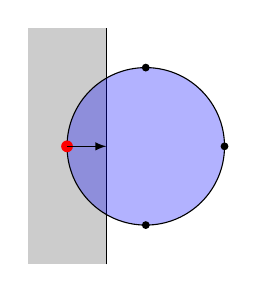
\begin{tikzpicture}[x=10mm,y=10mm]

    % Wall
    \fill[black!20!white] (-1.5, -1.5) rectangle (-0.5, 1.5);
    \draw (-0.5, -1.5) -- (-0.5, 1.5);

    % Ball
    \draw[fill=blue, fill opacity=0.3] (0, 0) circle (1);
    \node[fill, circle, inner sep=1pt] at ( 1, 0) {};
    \node[fill=red, circle, inner sep=1.5pt] at (-1, 0) {};
    \node[fill, circle, inner sep=1pt] at (0,  1) {};
    \node[fill, circle, inner sep=1pt] at (0, -1) {};

    % Arrow
    \draw[->,>=latex] (-1, 0) -- +(0.5, 0);
    \end{tikzpicture}
    \hspace{3em}
}
\hspace{1em}
\subfloat[Second collision check with the ball colliding with a wall corner]{
    \hspace{3em}
    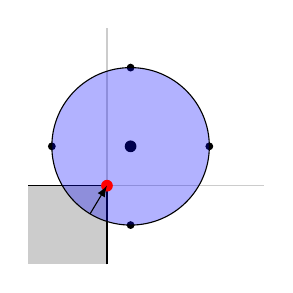
\begin{tikzpicture}[x=10mm,y=10mm]

    % Wall
    \fill[opacity=0.2] (-1.5, -1.5) rectangle (-0.5, -0.5);
    \draw[opacity=0.2] (-0.5, -1.5) -- (-0.5, 1.5);
    \draw[opacity=0.2] (-1.5, -0.5) -- (1.5, -0.5);
    \draw (-0.5, -1.5) -- (-0.5, -0.5) -- (-1.5, -0.5);

    % Ball
    \path (-0.2, 0) node[fill, circle, inner sep=1.5pt] (center) {}
        +(1, 0) coordinate (p)
            node[fill, circle, inner sep=1pt] at +( 1, 0) {}
            node[fill, circle, inner sep=1pt] at +(-1, 0) {}
            node[fill, circle, inner sep=1pt] at +(0,  1) {}
            node[fill, circle, inner sep=1pt] at +(0, -1) {};
    \node(ball) at (center)[draw, fill=blue, fill opacity=0.3, circle through=(p)] {};
    \node[fill=red, circle, inner sep=1.5pt] (corner) at (-0.5, -0.5) {};
    %\node[fill=red, circle, inner sep=1.5pt] (inwall) at (-1, -1) {};
    %\draw[opacity=0.1] (center) -- (inwall);


    % Arrow
    \draw[->,>=latex] (intersection of center--corner and ball) -- (-0.5, -0.5);
    \end{tikzpicture}
    \hspace{3em}
}
\subfloat{
    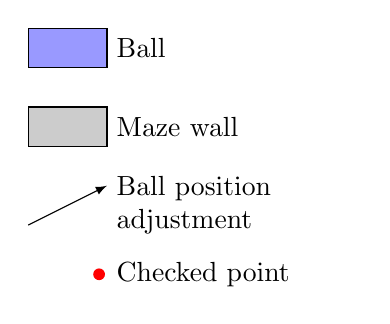
\begin{tikzpicture}[x=10mm,y=-5mm]

    \draw[fill=blue, fill opacity=0.4] (0, 0) rectangle +(-1, 1) +(0, .5)
        node[right, fill opacity=1] {Ball};
    \draw[fill, fill opacity=0.2] (0, 2) rectangle +(-1, 1) +(0, .5)
        node[right, fill opacity=1] {Maze wall};
    \draw[<-,>=latex] (0, 4) -- +(-1, 1); \draw (0, 4.5)
        node[right,text width=3cm, text badly ragged] {Ball position adjustment};
    \path(-0.1, 6.25) node[fill=red, circle, inner sep=1.5pt] {} +(0.1, 0)
        node[right] {Checked point};

    \end{tikzpicture}
}
\label{fig:collision-detection}
\caption{Ball collision detection}
\end{figure}

\section{Hardware}
\label{hw}

As part of the IT project, a prototype touchscreen was built.

\subsection{Operation and construction}

The touchscreen takes advantage of an optical phenomenon called
\emph{frustrated total internal reflection} (FTIR).
Light from infrared light-emitting diodes (LEDs) shines into a sheet of acrylic
glass.
Normally, this light is reflected repeatedly at the acrylic-air boundaries, so
that it effectively stays inside the acrylic.
When a finger is brought within a few wavelengths from the acrylic, it causes
the light to scatter away from the finger.

A camera placed behind the sheet of acrylic records the scattered light, and
the resuting image is processed to obtain \emph{blobs}, or areas corresponding
to the individual fingers touching the acrylic.
The particular camera used is a PlayStation Eye, favored by hobbyist
touchscreen builders for its low cost and high frame rate. % XXX: http://wiki.nuigroup.com/Cameras
The camera's infrared-blocking filter was replaced with a filter from an old
remote control.
The original lens was swapped for a wide-angle lens to reduce the needed depth
of the table.

To provide the infrared light, LEDs are soldered to form two strips.
Each strip is wrapped with clear adhesive tape for insulation, then aluminum
tape to reflect as much light as possible into the piece of acrylic.
The side facing the acrylic is kept clear of any tape.

A LCD (liquid crystal display) layer, obtained from a disassembled computer
monitor, is mounted behind the acrylic sheet.
As LCDs are transparent for infrared light, this does not affect the
touch-sensing capabilities of the screen.
However, the screen's backlight is not transparent and needed to be moved
behind the camera.
This results in decreased brightness when compared to a normal LCD.
Due to the construction of the LCD panel used, the camera could be inserted
into the original monitor chassis containing the backlight, with the lens
protruding through a hole in the backlight's diffuser.
The LED strips are wired to the LCD circuit board, sharing power from the
monitor's supply.

A sheet of tracing paper is installed % XXX: ?
behind the LCD. This serves both to blur the image or the camera so that it is
virtually invisible to the user, and in the reverse direction, to blur the
outside environment so that only blobs corresponding to touching fingers
are discernible by the camera.

The device is enlosed in a wooden box that blocks unwanted light from outside
and prevents movement of the camera relative to the display.
A hinged door in the back of the device allows inspection of the internals.
The power adaptor from the LCD monitor is secured inside the enclosure, away
from the backlight, so that the socket for a power cable is accessible.
In addition to the power cable, an USB cable for the camera and a VGA cable
for the monitor extend from the device and need to be connected to the computer
running the games.

\begin{figure}[p]\small
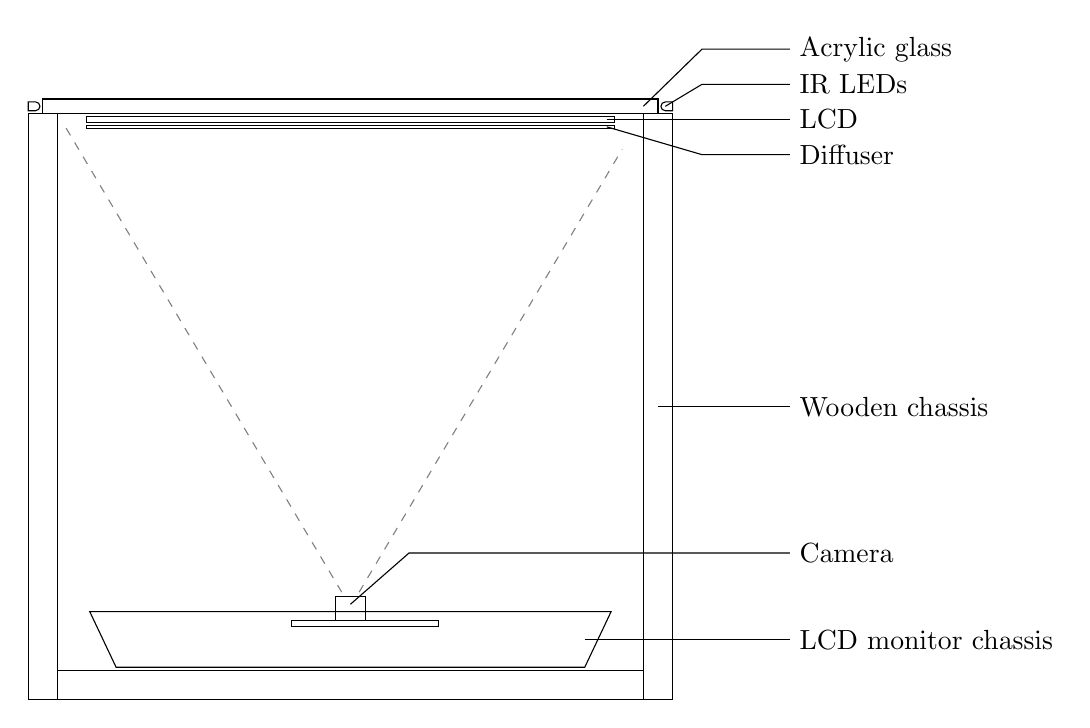
\begin{tikzpicture}[x=4mm,y=4mm,scale=0.93]
\draw (-.5,0) rectangle (20.5,.5); % acrylic
\draw (-1,0) rectangle (0,-20); % front wood
\draw (20,0) rectangle (21,-20); % back wood
\draw (0,-19) rectangle (20,-20); % bottom wood
\draw (1,-.1) rectangle (19,-.3); % LCD
\draw (1,-.4) rectangle (19,-.5); % diffuser
\draw (1.1,-17) -- (18.9,-17) -- (18,-18.9) -- (2,-18.9) -- cycle; % backlight
\draw (9.5,-16.5) rectangle (10.5,-17.3); % camera lens
\draw (8,-17.3) rectangle (13,-17.5); % camera body

\draw (-1,.1) -- (-.75,.1) arc (-90:90:.15) -- (-1,.4) -- cycle; % LED 1
\begin{scope}[xscale=-1,xshift=-80mm]
\draw (-1,.1) -- (-.75,.1) arc (-90:90:.15) -- (-1,.4) -- cycle; % LED 2
\end{scope}

\draw (20,.25) -- (22,2.2) -- (25,2.2) node[right] {Acrylic glass};
\draw (20.75,.25) -- (22,1) -- (25,1) node[right] {IR LEDs};
\draw (18.75,-.2) -- (22,-.2) -- (25,-.2) node[right] {LCD};
\draw (18.75,-.45) -- (22,-1.4) -- (25,-1.4) node[right] {Diffuser};
\draw (20.5,-10) -- (25,-10) node[right] {Wooden chassis};
\draw (10,-16.75) -- (12,-15) -- (25,-15) node[right] {Camera};
\draw (18,-17.95) -- (25,-17.95) node[right] {LCD monitor chassis};

% camera view lines?
\draw[gray,dashed,shorten >=5pt,shorten <=2pt] (9.8,-16.5) -- (0, 0);
\draw[gray,dashed,shorten >=15pt,shorten <=2pt] (10.2,-16.5) -- (20, 0);

\end{tikzpicture}
\label{fig:schem}
\caption{Schematic diagram of the touchscreen}
\end{figure}

\begin{figure}[p]\small
\subfloat[Front view of the inside]{
    \label{fig:box-front}\includegraphics[width=6.5cm]{box-open-front}}
\hspace{1em}
\subfloat[Touchscreen in action]{
    \label{fig:box-top}\includegraphics[width=6.5cm]{IMG_0950}}
\caption{Photographs of the touchscreen}
\end{figure}

\subsection{Problems}

Due to the decreased brightness of the LCD backlight, the touchscreen functions
best in rooms that are not fully lit.
Also, it reacts differently to fingers of different people, or even different
fingers on the same hand, which means that some people may need to press harder
on the screen than others.

The firmware and drivers for the PS3 Eye camera are designed to adapt to
lighting conditions.
Whenever such an adaptation occurs, “fake” tou\-ches may start being registered
or legitimate touches may be missed.
Keeping the table and room lit by a stable overhead light source helps prevent
this problem.

Despite these shortcomings, the table is usable and according to user testing,
the games played on it are quite engaging.

\newpage

\tableofcontents

\listoffigures

\end{document}

% XXX: Refer to all figures

